\documentclass[12pt]{article}
\usepackage[margin=1.3in]{geometry}
\usepackage{titlesec}
\usepackage{tikz}
\usepackage{tikz-qtree}
\usepackage{bm}

\title{Trabalho V}
\author{Bruno Samuel A. Gonçalves}
\date{}

\titleformat{\section}
  {\normalfont\Large\bfseries}{}{0em}{}

\begin{document}

\maketitle
\thispagestyle{empty}

\section{Questão 8}

\noindent Fórmula:

\[
    Q(x)\lor P(a)
\]

\noindent 1. Árvore de Sintaxe:

\begin{center}
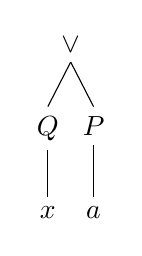
\begin{tikzpicture}
\Tree 
[.$\lor$
    [.$Q$
        $x$
    ]
    [.$P$
        $a$
    ]
]
\end{tikzpicture}
\end{center}

\noindent 2. Classificação:

\begin{center}
    \textbf{Verdadeira} \\
    $P(a) \to \bm{\top}$
\end{center}

\end{document}
